%
% This is Chapter 1 file (chap1.tex)
%
\chapter{Security Evaluation}
A pentesting report for the final project of CISC472. Hosted versions of the project can be found at:

https://banningcalvin-redchan.glitch.me/

and at :

https://github.com/banningcalvin/redchan/.


\section{Trivial Vulnerabilities}
These vulnerabilities will not result in data loss, but may result in an adverse user experience.
\begin{itemize}
    \item Users can comment or post very quickly and overload a post with comments.
    \item User emails are used to identify posts. This presents a potential breach of privacy.
    \item When logged in, upvotes do not appear, and multiple seem to appear from a single click. (A bug, perhaps?). I recall this system working at one point, so I'll have to investigate what is broken in order to implement an appropriate fix.
\end{itemize}

\section{Data Vulnerabilities}
It doesn't seem that there are any major vectors to leak data on the website. The login system could conceivably be fooled by copying over a valid auth token, but because all data is sent via https, I felt that such an attack would be unsuccessful. However, I did think that the way I was storing the token while browsing a page was insecure. If an attacker had access to the cookies on the machine, they could copy them over to another. While a new token is generated on navigation, and it is set to timeout at a reasonable interval, a quick execution could mean that an attacker could potentially steal another user's credentials temporarily.

Other than this, Firebase - which is used as a backend - does not make any content not already shown on the site public, so UID's, etc. are kept private as they should be.

\section{Testing of other vulnerabilities}
I briefly tried a variety of common attacks to see if the application was vulnerable:
\begin{itemize}
    \item Firebase is not vulnerable to SQL injection, and because all data is read only as plaintext and the way it is read into and out of Firebase.
    \item There do not seem to be any XSS vulnerabilities.
    \item I even found that glitch was not authorized to perform logins:\\
    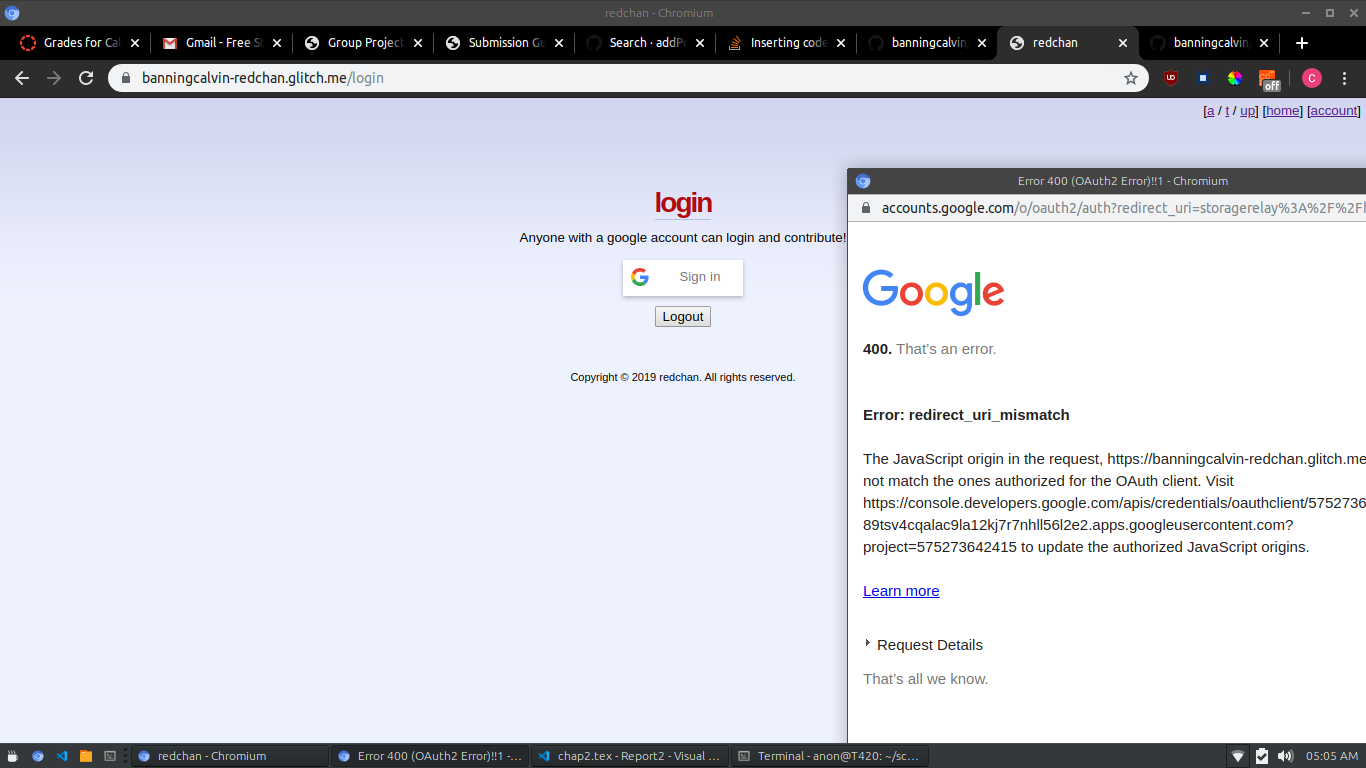
\includegraphics[width = 400pt]{images/account.png}\\
    This is a testament to how well authentication is setup.
    \item Role elevation seemed impossible because of Firebase rules. In order to gain permissions to, say, post on the /up/ board (where you must be a moderator), there is no other way than to have an account. This is because setting the moderator flag can only be done from Firebase. From a UX perspective, this isn't the best method. However, such a utility would be rarely used because moderators would vastly outnumber users, so it is a low-priority problem.
\end{itemize}

\section{Vulnerability Resolution}

There are three security concerns which ought to be addressed before release. First, users should be identified by an anonymous username, rather than their personal email. This is a simple fix: force users to choose a unique username when logging in for the first time, and associate this with their account. When making posts, lookup the user according to the UID returned by the auth operation, and assign their username to the post. Do not allow the user to pass in a username, as they could pass in any arbitrary name and make it seem as if it were posted by another user.

Second, the upvote system should be fixed. They should appear immediately, and users should only be able to have a power of 1 vote. I think this might be related to how Firebase structures upvotes, and a failure on my part to ensure each vote is associated with a unique UID. Preventing duplicate votes if a UID-vote pair is present would be the quickest fix.

Finally, storing the auth token in a cookie seems to be a moderate security concern. Although this token is always updated on navigation, the fact that it is stored as plaintext, even on a single machine, and only for a short time, means that a compromised machine is an attack surface. Of course, stealing credentials with a keylogger is just as likely and outside the scope of this application's security, but cookie theft through other means is possible. Rather than storing the token in a cookie, simply generate one whenever necessary, and do not save it.